% !TeX root = ../main.tex

\chapter{排序算法优化}

\section{排序算法的性能分析}
\subsection{传统十种排序算法的性能分析}
下面对十种传统的排序算法进行介绍和分析,主要的分析角度为时间复杂度、空间复杂度以及硬件友好程度。

\subsubsection{冒泡排序}
    冒泡排序的基本思想在于对数组重复遍历,逐个比较数组相邻元素的值并进行交换;当遍历完一遍以后,没有进行交换操作,即说明排序完成。对于冒泡排序来说,其时间复杂度为$O(n^2)$,空间复杂度为$O(1)$,就其本身而言,并没有并行性;但是基于其的改进算法,如奇偶排序,可以应用于并行计算。

\subsubsection{选择排序}
    选择排序基本思想为:首先从未排序的数组中遍历,选出最小(大)的数放在排序数组的起始位置;再从剩余未排序的数组中选择最小(大)的数,放在已排序数组的末尾,以此往复,直到将未排序数组完全遍历。在实际操作过程当中,通常将数组的前$n$位作为有序数组,当进行第$n+1$次遍历时,从第$n+1$位元素开始,选出最小(大)的数,再将其与第$n+1$个数进行交换,从而形成长度为$n+1$的有效数组。选择排序的时间复杂度为$O(n^2)$,空间复杂度为$O(1)$。

\subsubsection{插入排序}
    插入排序的思想是通过对数组中已经完成排序的有序数列进行扫描,将未排序的数据插入到已排序序列当中。和冒泡排序和选择排序类似,插入排序的时间复杂度也是$O(n^2)$,空间复杂度为$O(1)$。

\subsubsection{堆排序}
    堆排序的主要思想是通过不断的构建大顶堆,并提取堆顶的根节点,实现对于数组的排序。堆排序的步骤为:首先将待排序数组构造成一个大顶堆,再将堆顶元素和堆底元素进行对调,此时末尾元素即为最大值。再将剩余的$n-1$的元素重新构造成大顶堆,按照之前的步骤反复执行,即可得到一个有序数列。在堆排序中,初始构造堆的过程的时间复杂度为$O(n)$,接下来交换堆顶堆底元素并重新构造堆的过程,每次操作的时间复杂度为$O(\log n)$,重复$n$次,故全过程的时间复杂度为$O(n+n\log n)=O(n\log n)$。

\subsubsection{归并排序}
    归并排序针对于两个有序数列进行排序。在两个有序数列中分别设置指针,初始时二者分别指向两个有序数组的第一个元素,比较两个元素,选择较小者放入合并空间中,并移动该元素所在序列的指针;重复上述操作,直到所有元素均被放入合并空间当中。对于归并排序来说,如果有$n$个数需要排序,则需要进行$\log n$次归并操作,每次归并操作的时间复杂度为$O(n)$,所以归并排序的时间复杂度为$O(n\log n)$。归并排序的特点使其具有并行化的可能,对于每一层的归并排序,都可以将其并行化。关于归并排序的并行化我们会在后面详细阐述。

\subsubsection{快速排序}
    快速排序的思想在于每次排序时,从数列中挑出一个元素作为基准值,将小于基准值的数放在它的前面;将大于基准值的数放在它的后面,然后递归地将小于基准值的元素的子序列和大于基准值元素的子序列进行排序,从而最后形成有序数列。对于快速排序来说,其时间复杂度可以通过递归的方式求得。设快速排序的时间复杂度为$T(n)$,则一次单独的排序步骤的需要进行$O(n)$次操作,而剩下的时间由两个较小的子序列的排序时间复杂度决定,即$2T(n/2)$,故可得关系式$T(n)=O(n)+2T(n/2)$,从而解得$T(n)=O(n\log n)$。快速排序的空间复杂度为$O(\log n)$。

\subsubsection{希尔排序}
    希尔排序通过以一定步长交换不相邻的元素进行排序,每次排序减小步长,直到最后的步长为1。希尔排序可以看做改进版的插入排序,其最优时间复杂度通常为$O(n\log^2n)$,平均时间复杂度为$O(n^{1.3\sim 2})$,空间复杂度为$O(1)$。

\subsubsection{计数排序}
    计数排序首先找出数组中最大和最小的元素,然后统计数组中每个值为$i$的元素出现的次数,存入新开辟的数组当中,并且对每个值出现的次数进行统计,最后反向填充目标数组。由于计数排序并不是比较排序算法,所以其时间复杂度和空间复杂度都是为$O(n+m)$,其中$m$为数组的最小值和最大值的差值。

\subsubsection{桶排序}
    桶排序可以看做是一种改进的计数排序算法,其通过将数组按照值的范围放在不同的桶中,再在每个桶的内部进行排序,所以其的时间复杂度为$O(n+m)$,空间复杂度为$O(m\times n)$,其中$m$为桶的数目。

\subsubsection{基数排序}
    基数排序的基本思想在于按顺序对数的每一位进行排序。如对于十进制数组排序,首先根据各个数的个位数的值,将其放在十个“桶”当中,然后依次取出完成一次排序;再根据各个数的十位数的值,再将其放入十个桶当中,依次取出,如此往复,直到完成对于最高位的排序,按顺序取出的数组即为完成排序的数组。由基数排序的算法可以看出,它的时间复杂度仅仅取决于数的位数以及数组长度。因此,其时间复杂度为$O(k\times n)$,其中$k$为数的位数。
    

综上,各种排序算法的时间复杂度、空间复杂度如表\ref{table:algorithm}所示。
\begin{table}[htbp]
\centering
\caption{各种排序算法的时间复杂度、空间复杂度}
\setlength{\tabcolsep}{16mm}{
\begin{threeparttable}
\begin{tabular}{ccc}
\toprule
排序算法 & 时间复杂度          & 空间复杂度      \\
\midrule
冒泡排序 & $O(n^2)$       & $O(1)$          \\
选择排序 & $O(n^2)$       & $O(1)$         \\
插入排序 & $O(n^2)$       & $O(1)$             \\
堆排序  & $O(n\log n)$   & $O(1)$             \\
归并排序 & $O(n\log n)$   & $O(n)$      \\
快速排序 & $O(n\log n)$   & $O(\log n)$        \\
希尔排序 & $O(n\log^2n)$   & $O(1)$             \\
计数排序\tnote{1} & $O(n+m)$       & $O(n+m)$          \\
桶排序\tnote{2}  & $O(n+m)$         & $O(m\times n)$            \\
基数排序\tnote{3} & $O(k\times n)$ & $O(k+n)$         \\
\bottomrule
\end{tabular}
\begin{tablenotes}
        \footnotesize
        \item[1] 计数排序中,m代表数据的最大值减最小值。
        \item[2] 桶排序中,m代表桶的个数。
        \item[3] 基数排序中,k代表数值中的``数位"个数。
\end{tablenotes}
\end{threeparttable}}
\label{table:algorithm}
\end{table}

\subsection{k路归并算法}
除了以上传统的排序算法,我们还想介绍一种特殊的排序算法——k路归并算法。k路归并算法指的是利用归并排序的思想,对k输入数列进行排序的算法。k路排序算法有很多变种,接下来我们进行逐一介绍和分析。
\subsubsection{传统多路归并排序}
\begin{figure}[htbp]
    \centering
    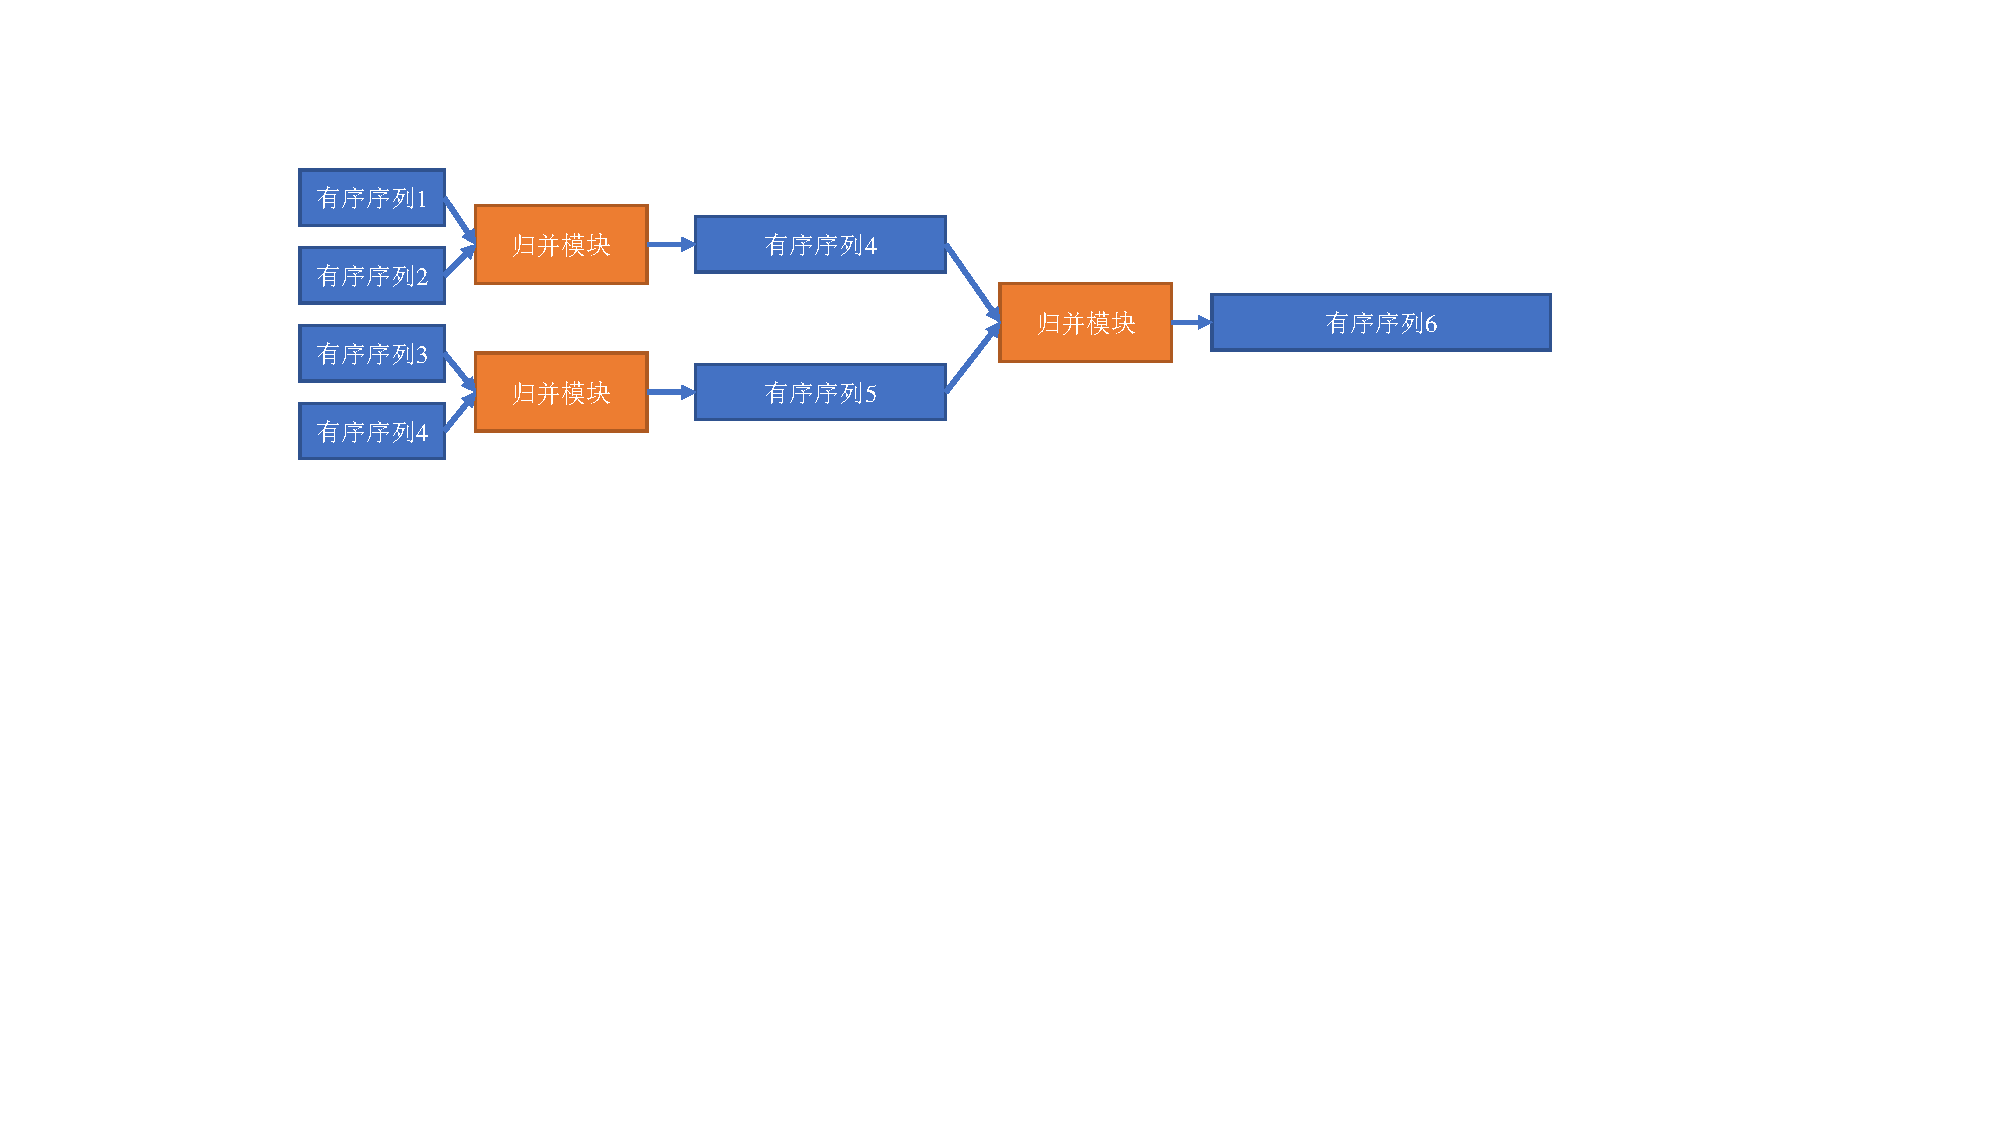
\includegraphics[width=\linewidth]{figures/traditional k way sort.pdf}
    \caption{4路归并排序示意}
    \label{fig:traditional_k_way_sort}
\end{figure}
传统归并排序采用的``Divide and Conquer"(分治法)进行排序,先将待排序数组分成等量子数组进行排序,分别形成有序数列。然后对有序数列进行排序形成更长的有序数列,不断重复,直到待排序数组完全有序。对于传统的k路排序来说,我们可以直接利用归并排序的``Conquer"部分,即对k个有序数列进行两两排序,不断归并直到最后将k个有序数列归并成一个有序数列。传统k路排序的整体思路如图\ref{fig:traditional_k_way_sort}所示。

\subsubsection{败(胜)者树归并}
除了上述的传统归并排序,还有一种多路归并方法被广泛使用:败(胜)者树。败者树的思想在于首先将每个输入的有序序列的最小元素取出,根据其大小构建败者树。败者树的叶子结点(即ls数组)记录败者序列编号,使得较小数(胜者)能够不断爬升比较,直到根节点,此时败者树的根节点记录的序列编号的中的第一个数即为全输入序列中最小的数。将其取出放在输出有序数列第一位,在不断重复此过程,直到所有输入序列均已排序完成。败者树的工作过程如图\ref{fig:loser_tree}所示。在这个例子当中,第一次构建败者树的过程将输入序列3的第一个元素6取出,然后序列3中元素前进一位。第二次建树的过程将输入序列1的第一个元素9取出,作为输出有序序列的第二个元素,由此不断循环,即可得到五个输入序列的整体的有序数列。胜者树的思想和败者树类似,只是在建树过程中,叶子结点记录的是胜者的序列编号,使得败者能够不断上浮。胜者树构建出来的有序序列是逆序(从大到小)的。
\begin{figure}[htbp]
    \centering
    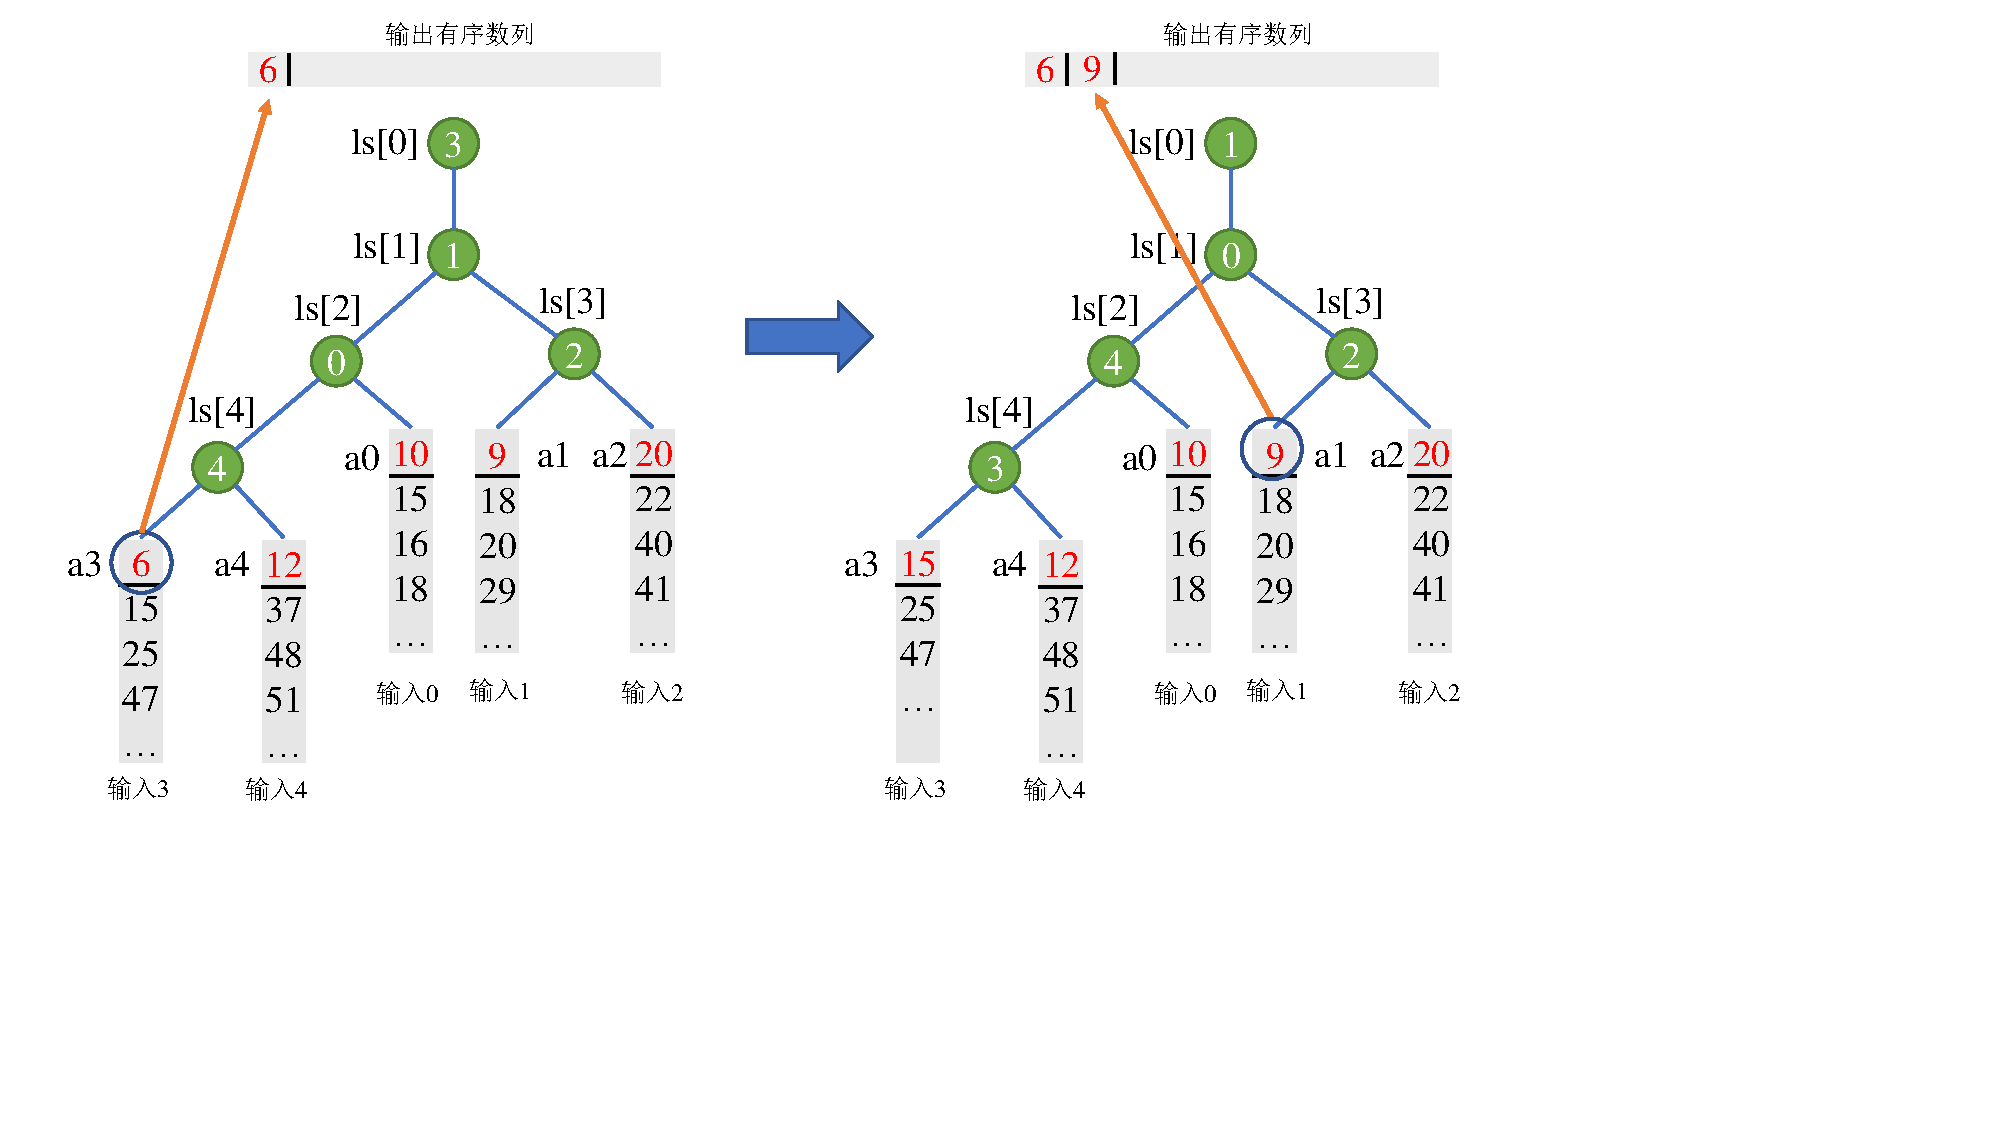
\includegraphics[width=\linewidth]{figures/loser_tree.pdf}
    \caption{败者树示意图}
    \label{fig:loser_tree}
\end{figure}


\section{针对大型数据集的排序算法所面临的问题}\label{facing_problems}

相对于小型数据集,要想针对面向大型数据集的排序算法进行加速,我们会遇到如下问题:
\begin{enumerate}
    \item 对于大型数据集来说,FPGA的片上资源无法一次性存储所有的数据,这就要求硬件加速架构必须分块从DRAM当中加载数据,这也会导致同时排序的过程中不可能一次性全部排序完成,只能先将每批次序列的数据排成有序数组,再对这些有序数组进行排序。
    \item 对于大型数据集来说,即使是分批次载入数据,如果每个批次的数据量仍然较大,且硬件上面没有充分流水化/并行化的话,可能会造成严重的数据依赖,即排序过程中的每次循环过程都会很长,且直到该轮循环完成之前,下一轮循环都无法开始。这就会导致极高的延迟,从而大大影响硬件性能。
    \item 对于大型数据集来说,算法本身的时间复杂度会极大地影响其效率,因此,我们需要比较不同时间复杂度的增长趋势,如图\ref{fig:time complexity}所示。图中,横坐标表示待排序数的个数,纵坐标表示的事相对的时间复杂度,该图显示了$O(n^2)$,$O(n\log n)$,$O(n\log^2n)$, $O(kn)$ 时间复杂度的增长趋势。从图中可以看到,当$n$足够大时,$O(n\log n)$,$O(kn)$的增长速度明显要慢于其他的函数,因此,我们可以仅选择时间复杂度为$O(n\log n)$和$O(kn)$的算法,即堆排序、归并排序、快速排序以及基数排序。至于计数排序和桶排序,由于其时间复杂度和空间复杂度都取决于数据的最大值和最小值之差,当要排序的数据的最大值和最小值之差很大时(对于我们讨论的情形,待排序数据位宽为32),其所需的时间和存储空间都是巨大的,因此我们不将其放入讨论范围。
\end{enumerate}
\begin{figure}[htbp]
    \centering
    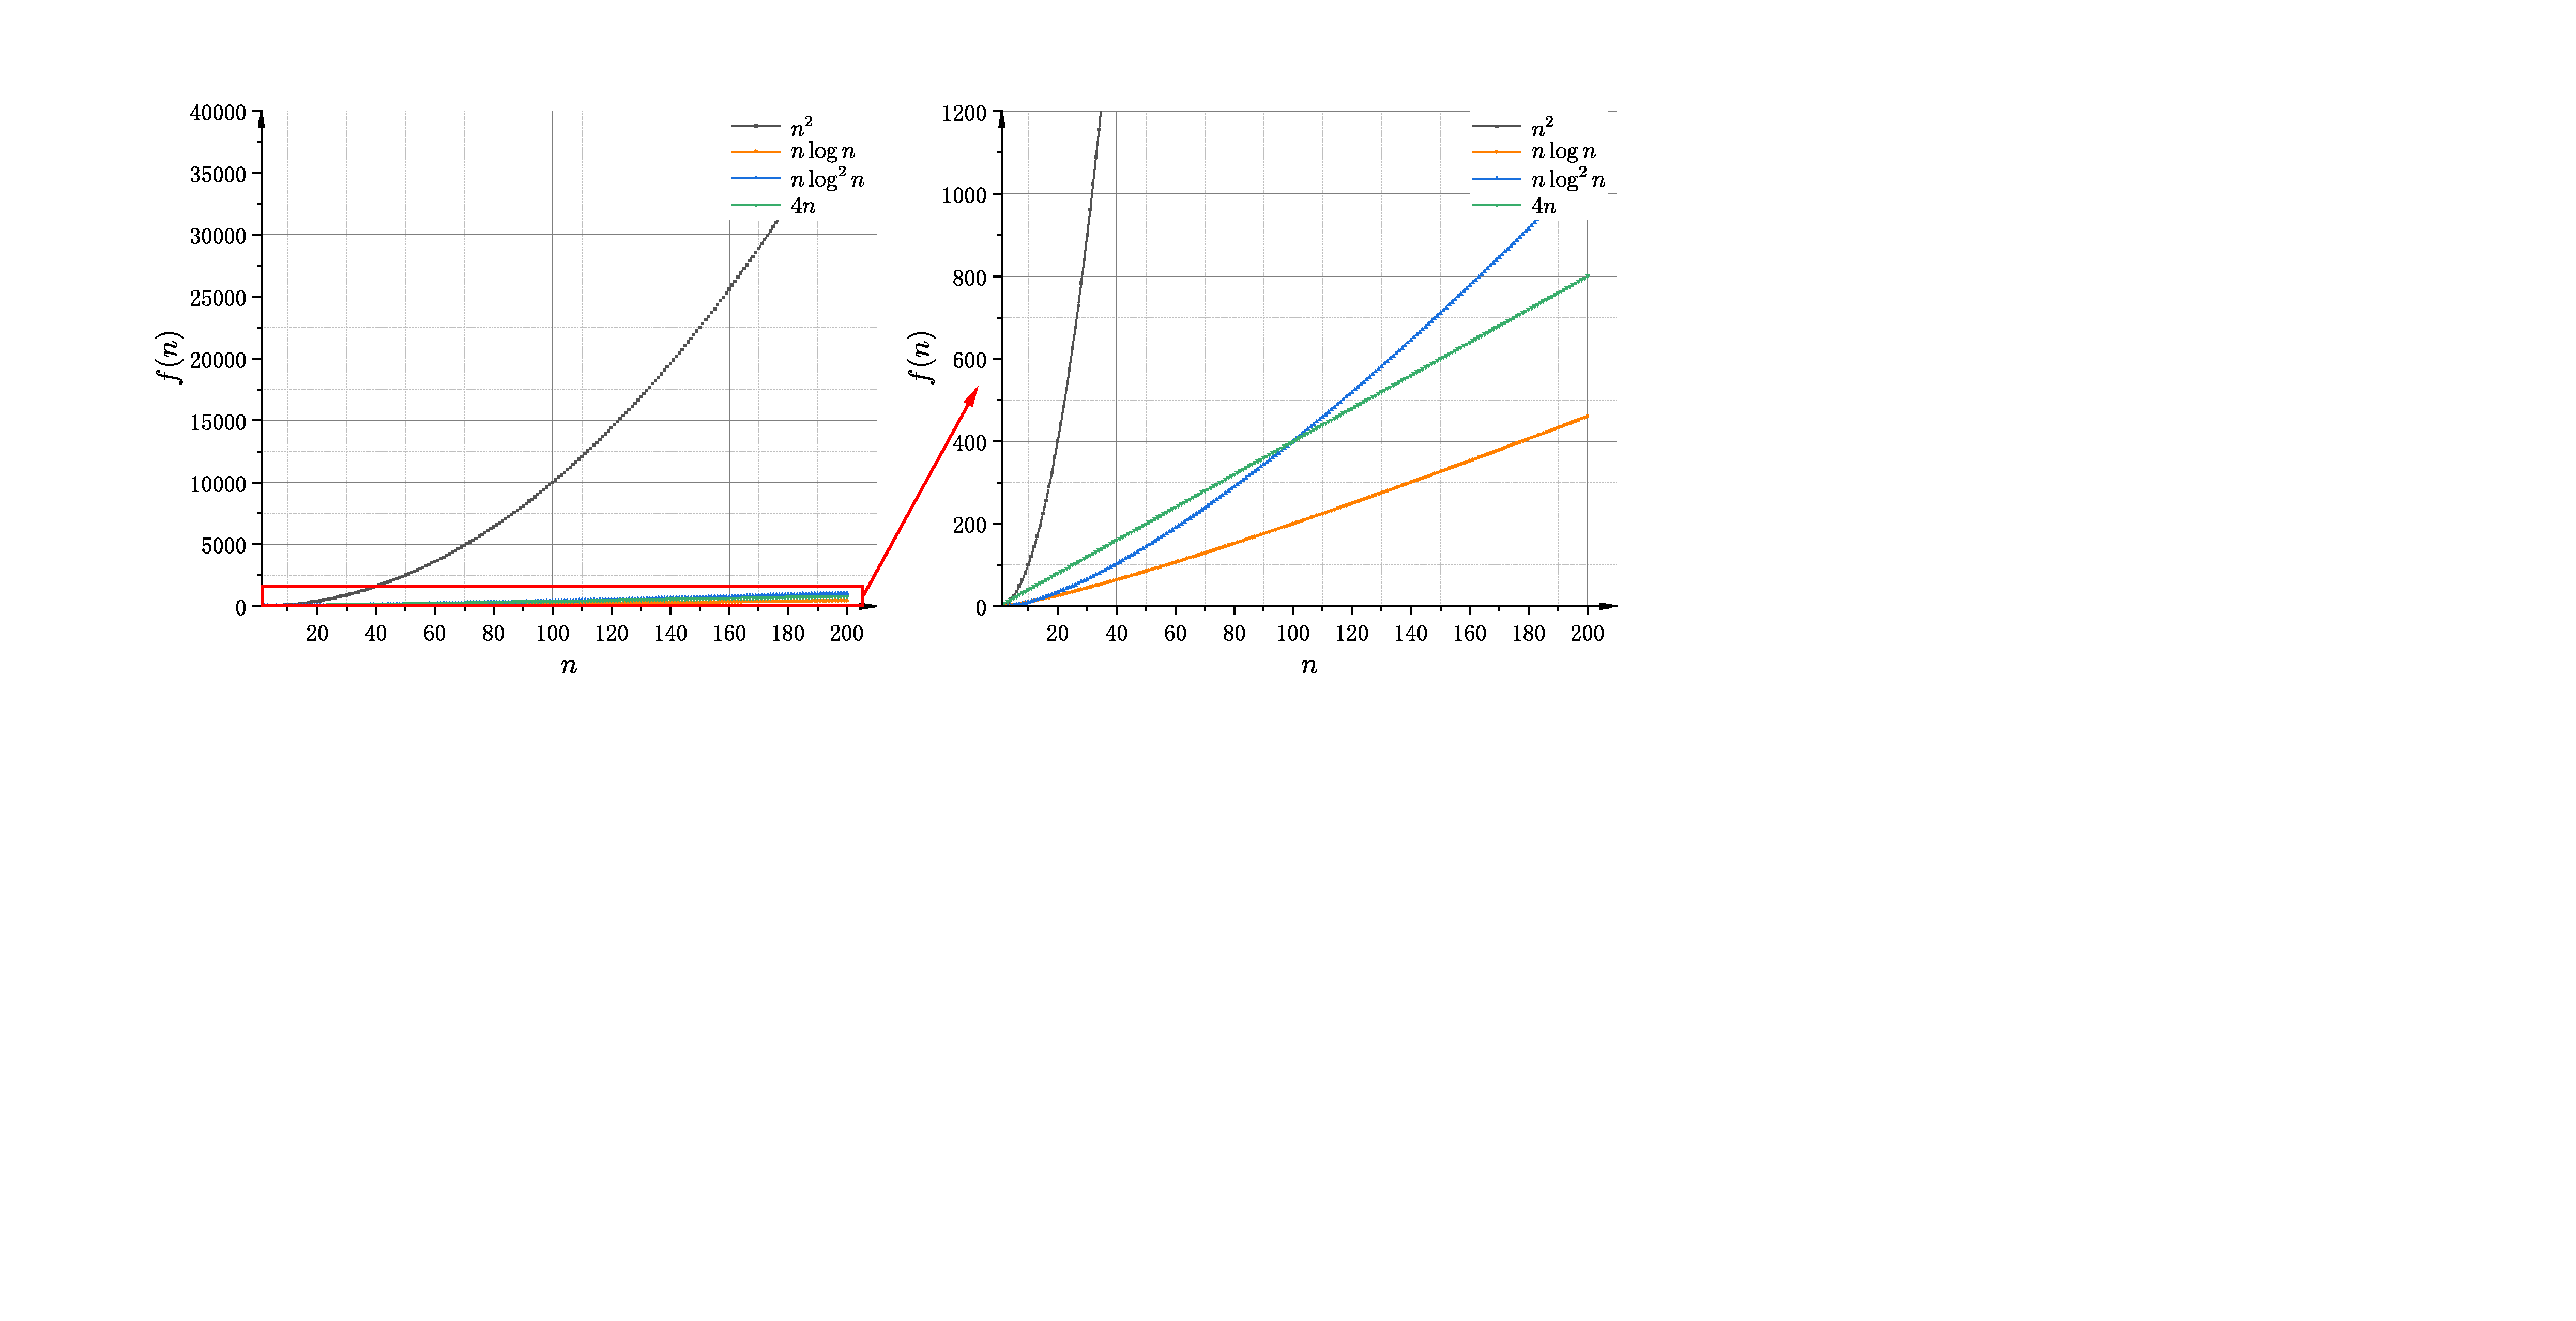
\includegraphics[width=\linewidth]{figures/time complexity.pdf}
    \caption{各个算法时间复杂度增长趋势}
    \label{fig:time complexity}
\end{figure}


\section{面向硬件的排序算法优化策略}

大部分排序算法都需要用到嵌套循环语句。因此从硬件的角度,对于循环的优化必不可少。同时,HLS提供了丰富的硬件优化策略来降低延迟以及提升吞吐量。下面我们选取几个常用的硬件优化策略进行介绍。

\subsection{对于循环的优化策略}
\subsubsection{循环分块(Loop Tiling)}
\begin{figure}[htbp]
    \centering
    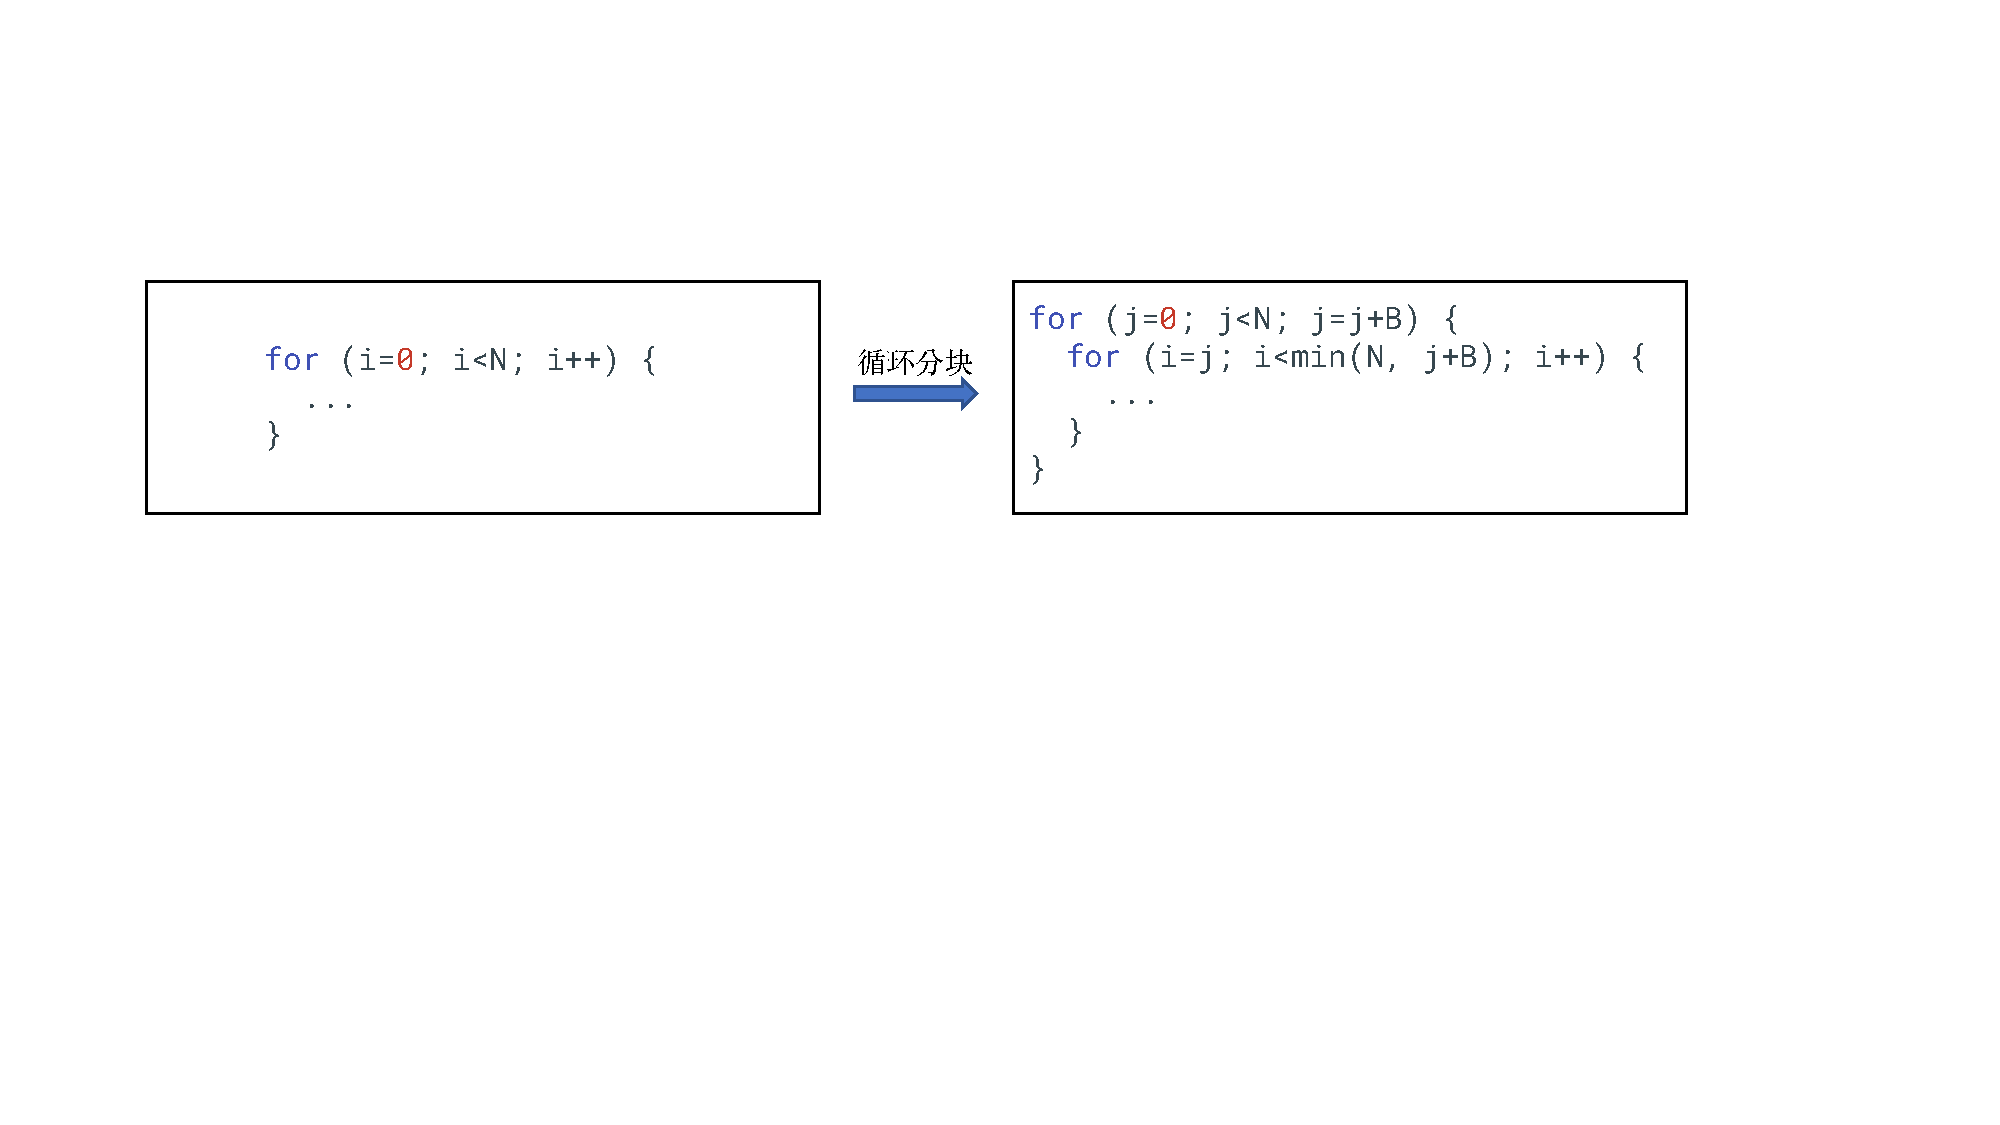
\includegraphics[width=\linewidth]{figures/loop tiling.pdf}
    \caption{循环分块算法示意}
    \label{fig:loop_tiling}
\end{figure}

循环分块通过将“迭代空间”分割成更小的块,来确保循环中使用的数据被重复利用之前能够一直保留在cache中,防止因为单次循环过长导致要复用的数据被移出cache。其算法的主要思想如图\ref{fig:loop_tiling}所示。在HLS当中,循环分块可以直接在C语言文件中进行修改,而不需要额外插入HLS pragma语句。


\subsubsection{循环交换(Loop Interchange)}
\begin{figure}[htbp]
    \centering
    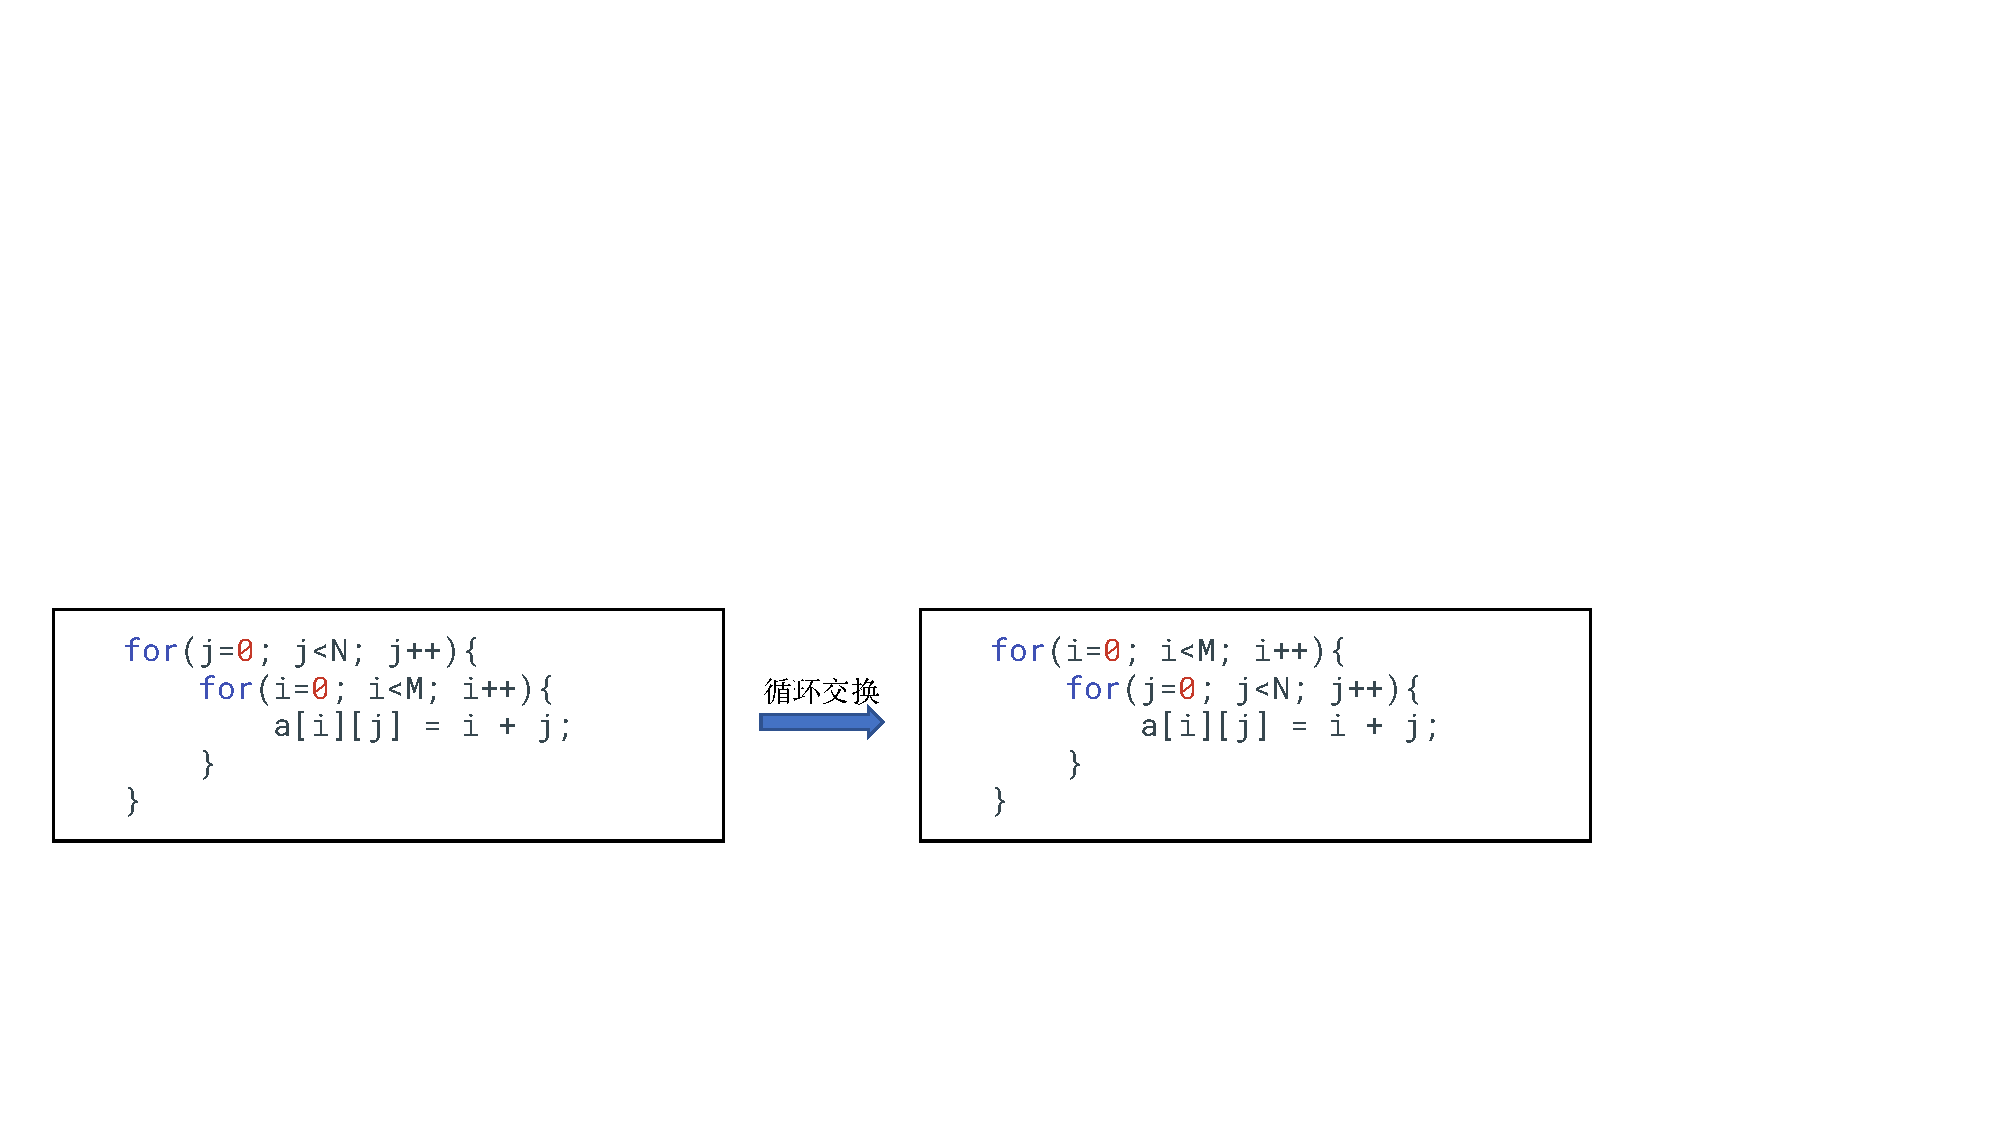
\includegraphics[width=\linewidth]{figures/loop interchange.pdf}
    \caption{循环交换算法示意。左图为行优先顺序遍历,右图为列优先顺序遍历}
    \label{fig:loop_interchange}
\end{figure}
循环交换即通过交换内外循环的顺序,使得代码具有更好的空间局部性。因为在C语言中,数据是以行优先的形式存储在cache当中的,所以在设计嵌套循环的时候,应该尽量以行优先遍历数据,从而达到更好的空间局部性。
\subsubsection{循环合并(Loop Fusion / Loop Merge)与循环分割(Loop Fission)}
\begin{figure}[htbp]
    \centering
    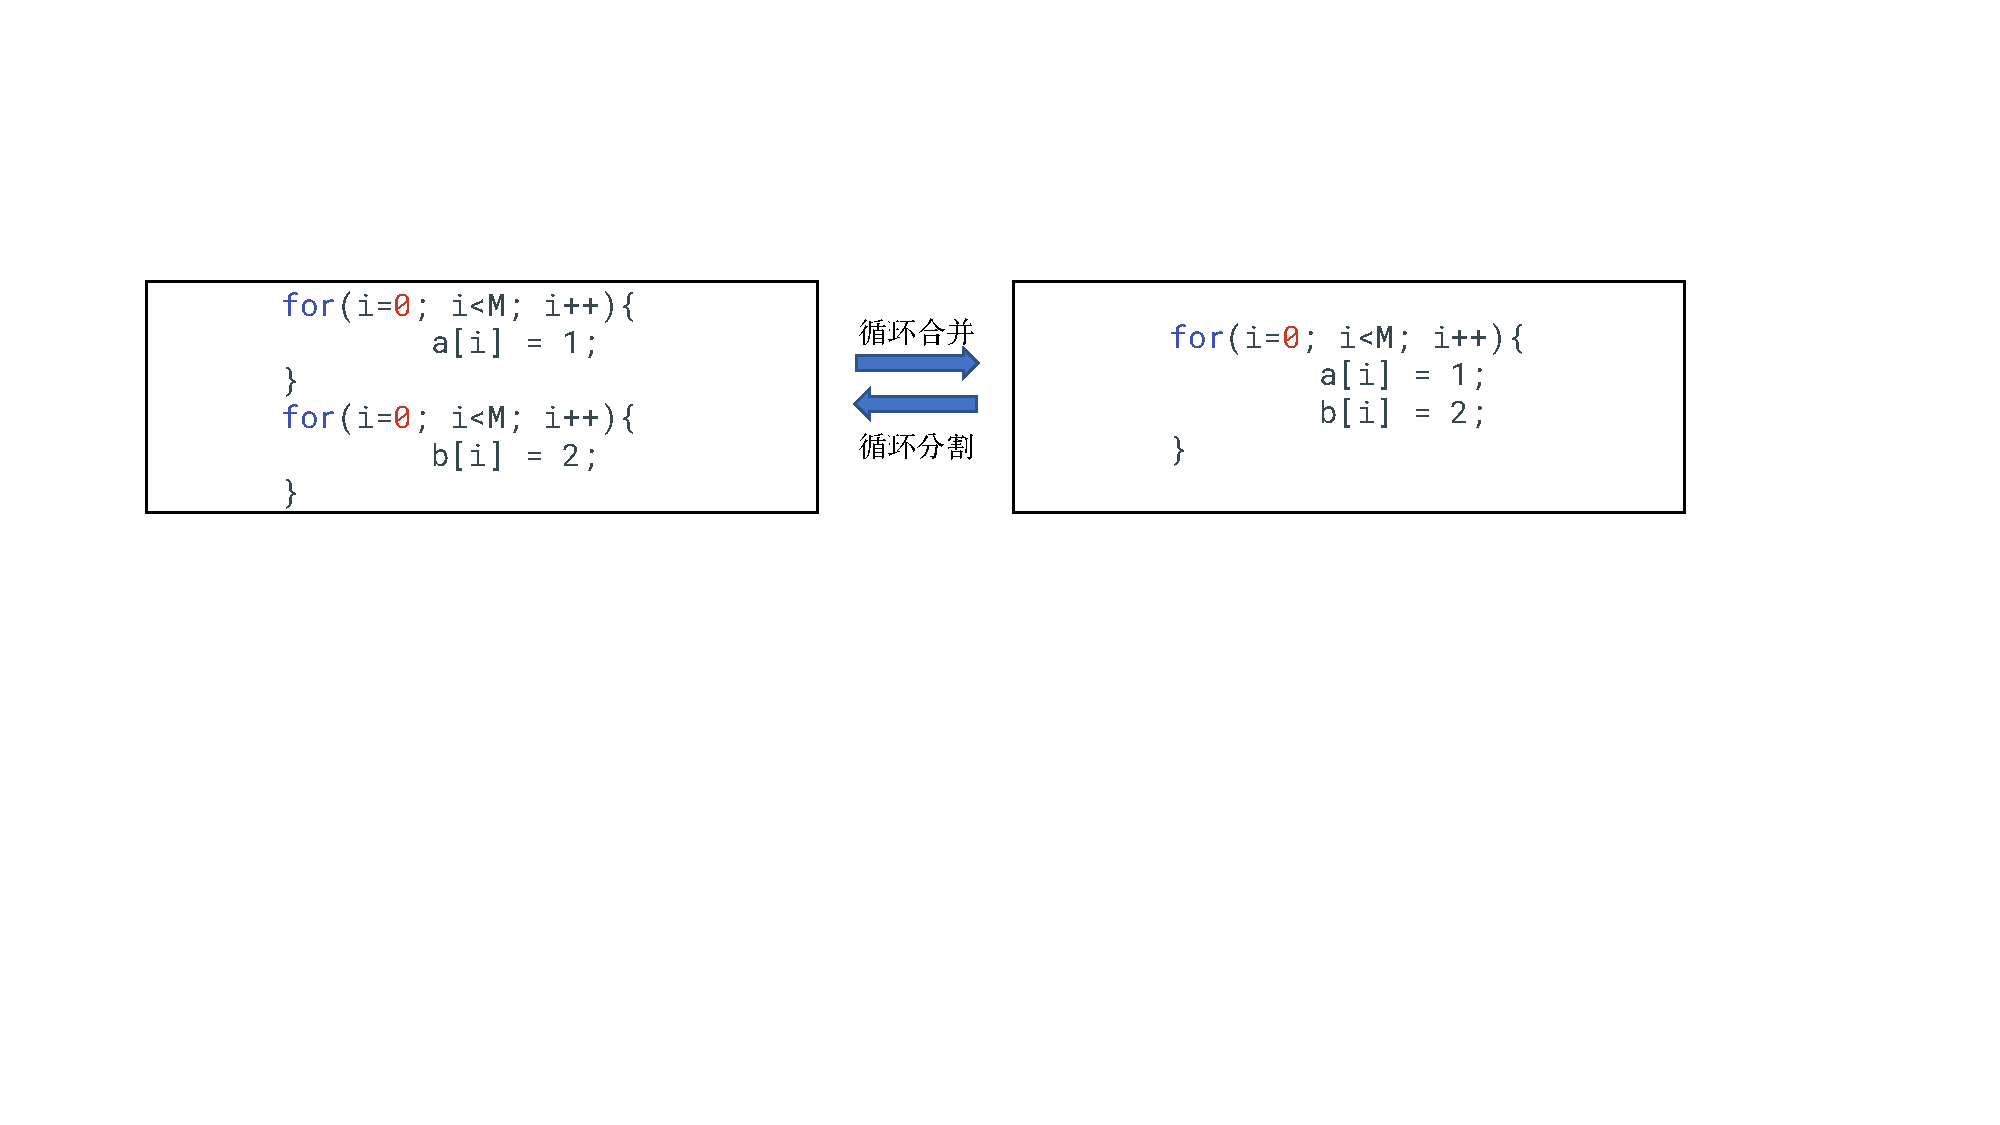
\includegraphics[width=\linewidth]{figures/loop fusion.pdf}
    \caption{循环合并与循环分割算法示意}
    \label{fig:loop_fusion}
\end{figure}
循环合并即将多个独立的循环过程合并到一个循环当中,而循环分裂则是相反的过程,将一个循环分割成多个独立的循环过程。循环合并通常是为了减少在多个循环中数据被重复利用的情形下,cache miss的概率,提升空间局部性,同时降低了循环控制结构的开销,消除可能存在的冗余分配,从而提升性能。在HLS当中,可以在循环语句之前添加\verb|#pragma HLS loop_merge|来实现循环合并,并尽可能并行化。
\subsubsection{循环展开(Loop Unrolling)}
\begin{figure}[htbp]
    \centering
    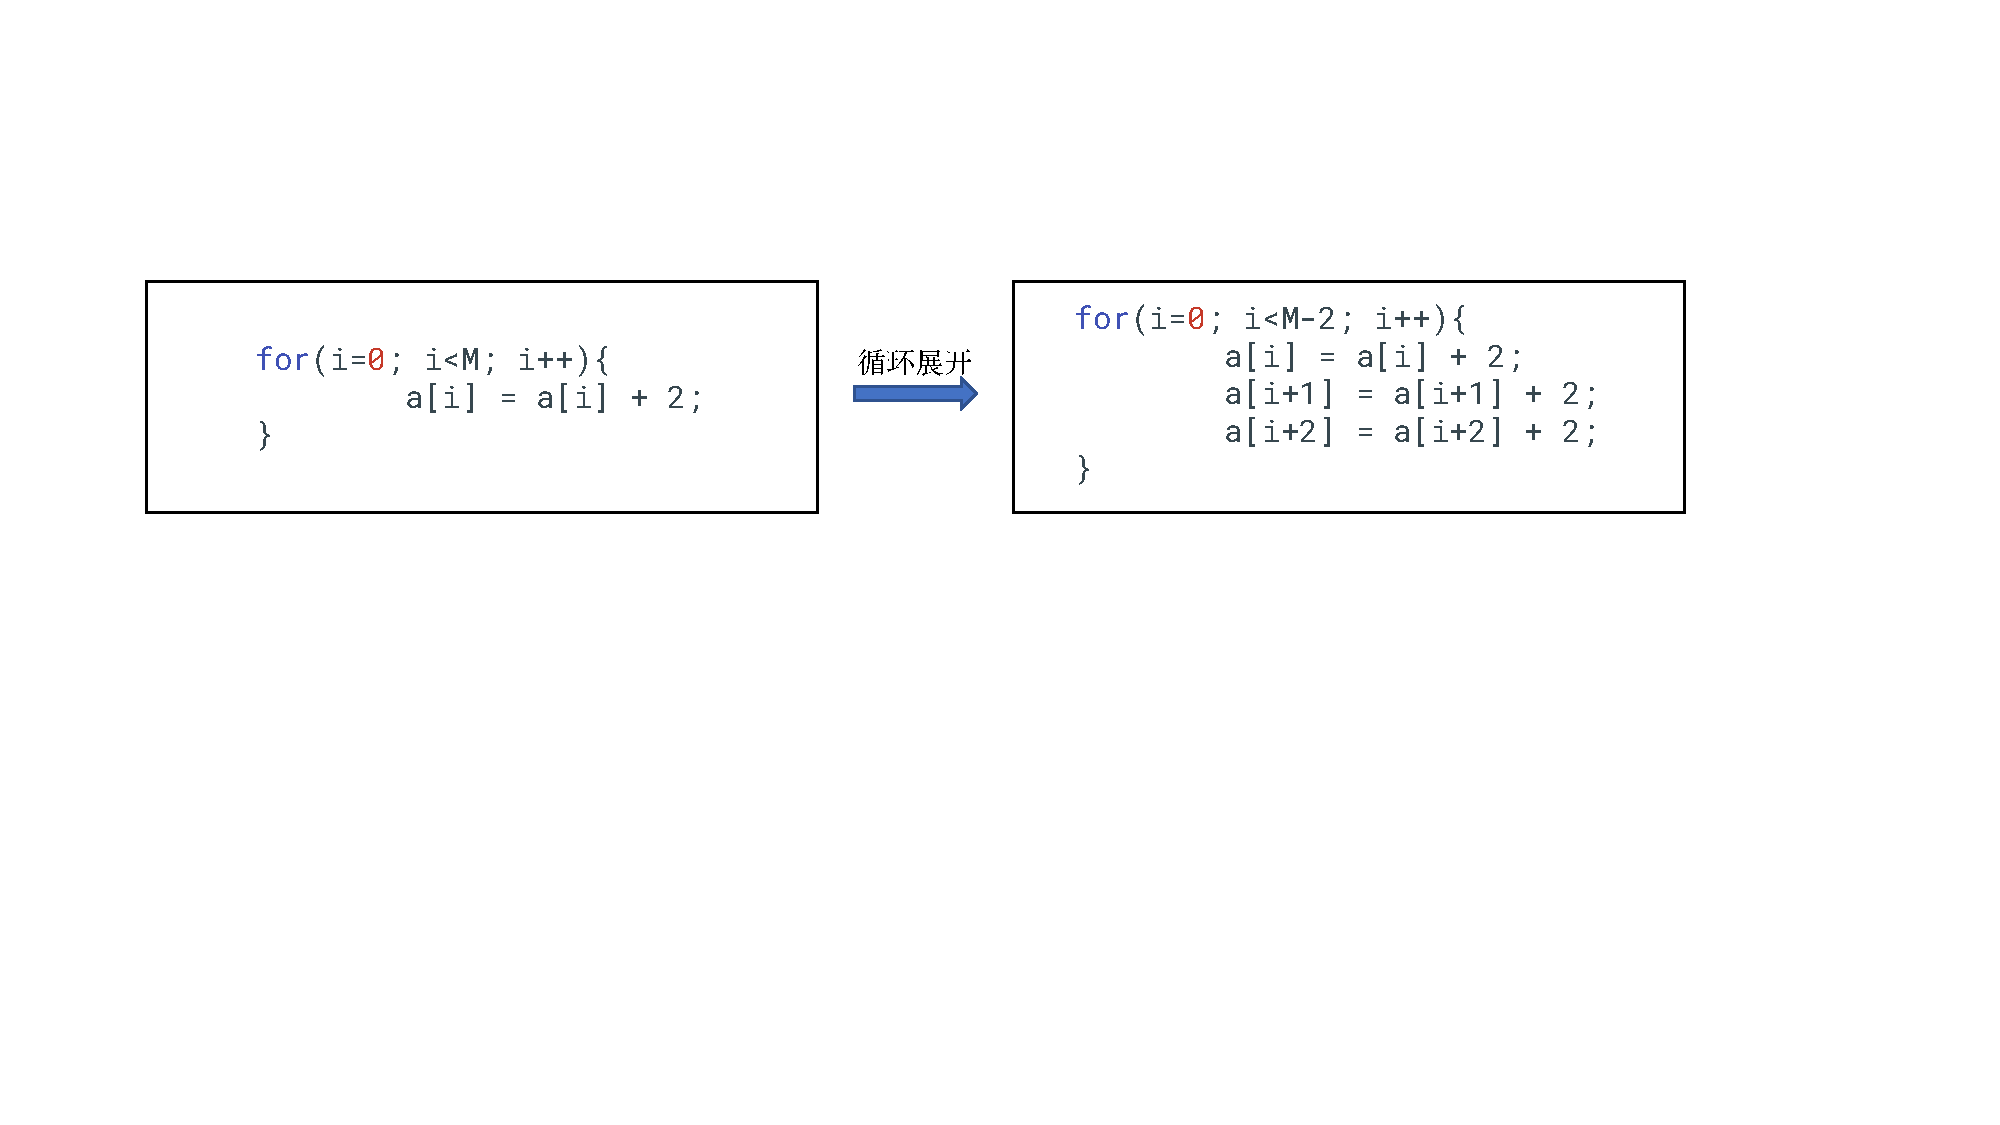
\includegraphics[width=\linewidth]{figures/loop unrolling.pdf}
    \caption{循环展开算法示意}
    \label{fig:loop_unrolling}
\end{figure}
循环展开通过提升每次循环中执行的操作数量来减少循环次数,降低分支预测的错误概率。同时,在HLS当中,通过循环展开,如果没有数据相关,每个循环内的操作可以并行执行,从而提升了并行度以及处理速度。在HLS当中,可以在需要展开的循环前面添加\verb|#pragma HLS unroll|来将循环展开。

\subsubsection{循环扁平化(Loop Flattening)}
\begin{figure}[htbp]
    \centering
    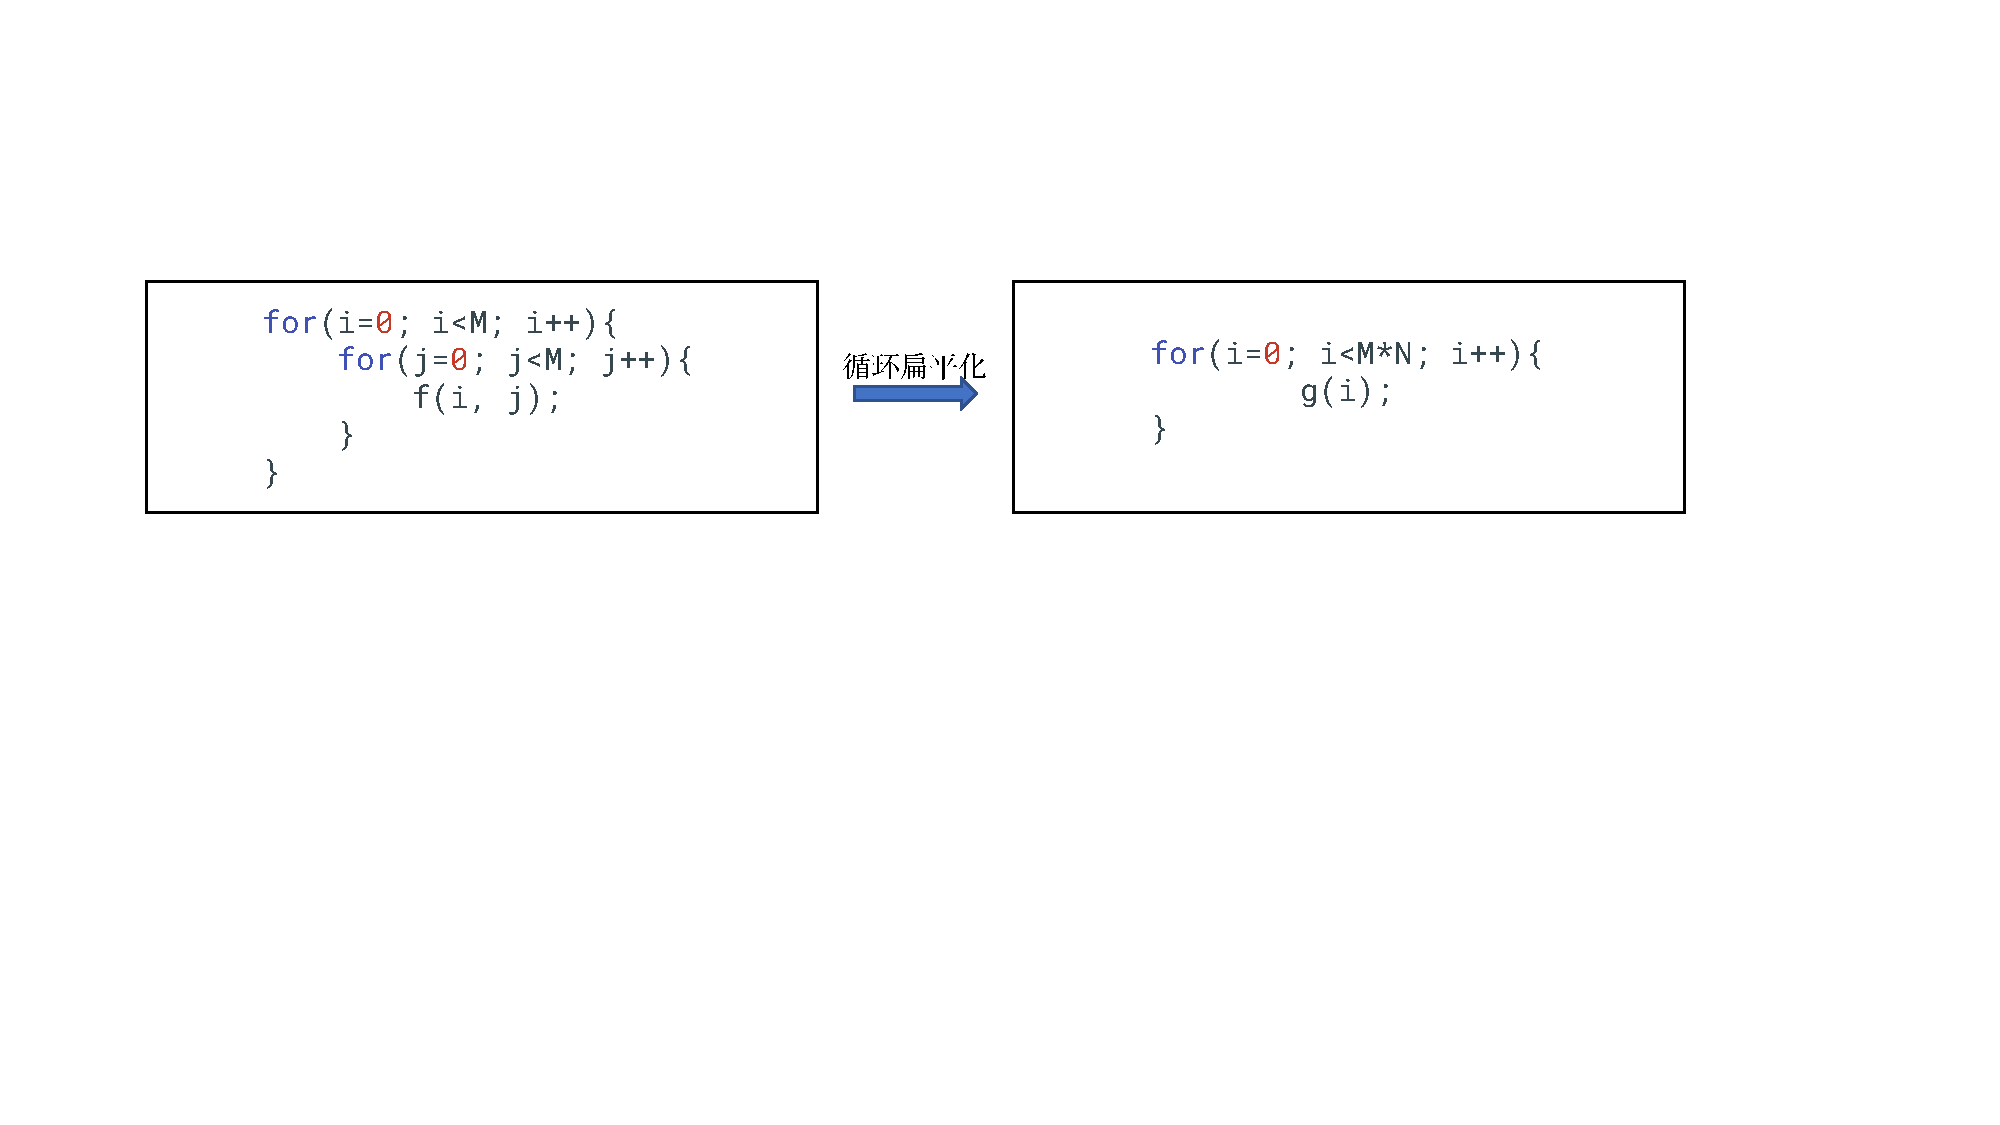
\includegraphics[width=\linewidth]{figures/loop flattening.pdf}
    \caption{循环扁平化算法示意}
    \label{fig:loop_flattening}
\end{figure}
循环扁平化将多层嵌套循环转为单层循环。从而能够更好的降低延迟和吞吐率。在HLS当中,可以在循环前面加上\verb|#pragma HLS loop_flatten|来将循环扁平化。
\subsection{流水线}

流水线是一种常用的提升架构并行度以及吞吐率的措施,其主要思想在于将程序分解成几个独立的阶段,每个阶段互不干扰,每个阶段对应一个硬件模块来处理。以最简单的五段流水线举例,它将计算机执行指令的过程分为了取指令、译码、执行、访存和写回五个过程,当流水线被填满时,所有的阶段都在执行不同的指令,而不会互相干扰,从而达到了降低硬件资源开销,提升处理器的时钟频率和性能。Vitis HLS提供了多细粒度的流水线选项,下面我们取最常用的指令级别流水线和任务级别流水线进行介绍。


\begin{figure}[htbp]
    \centering
    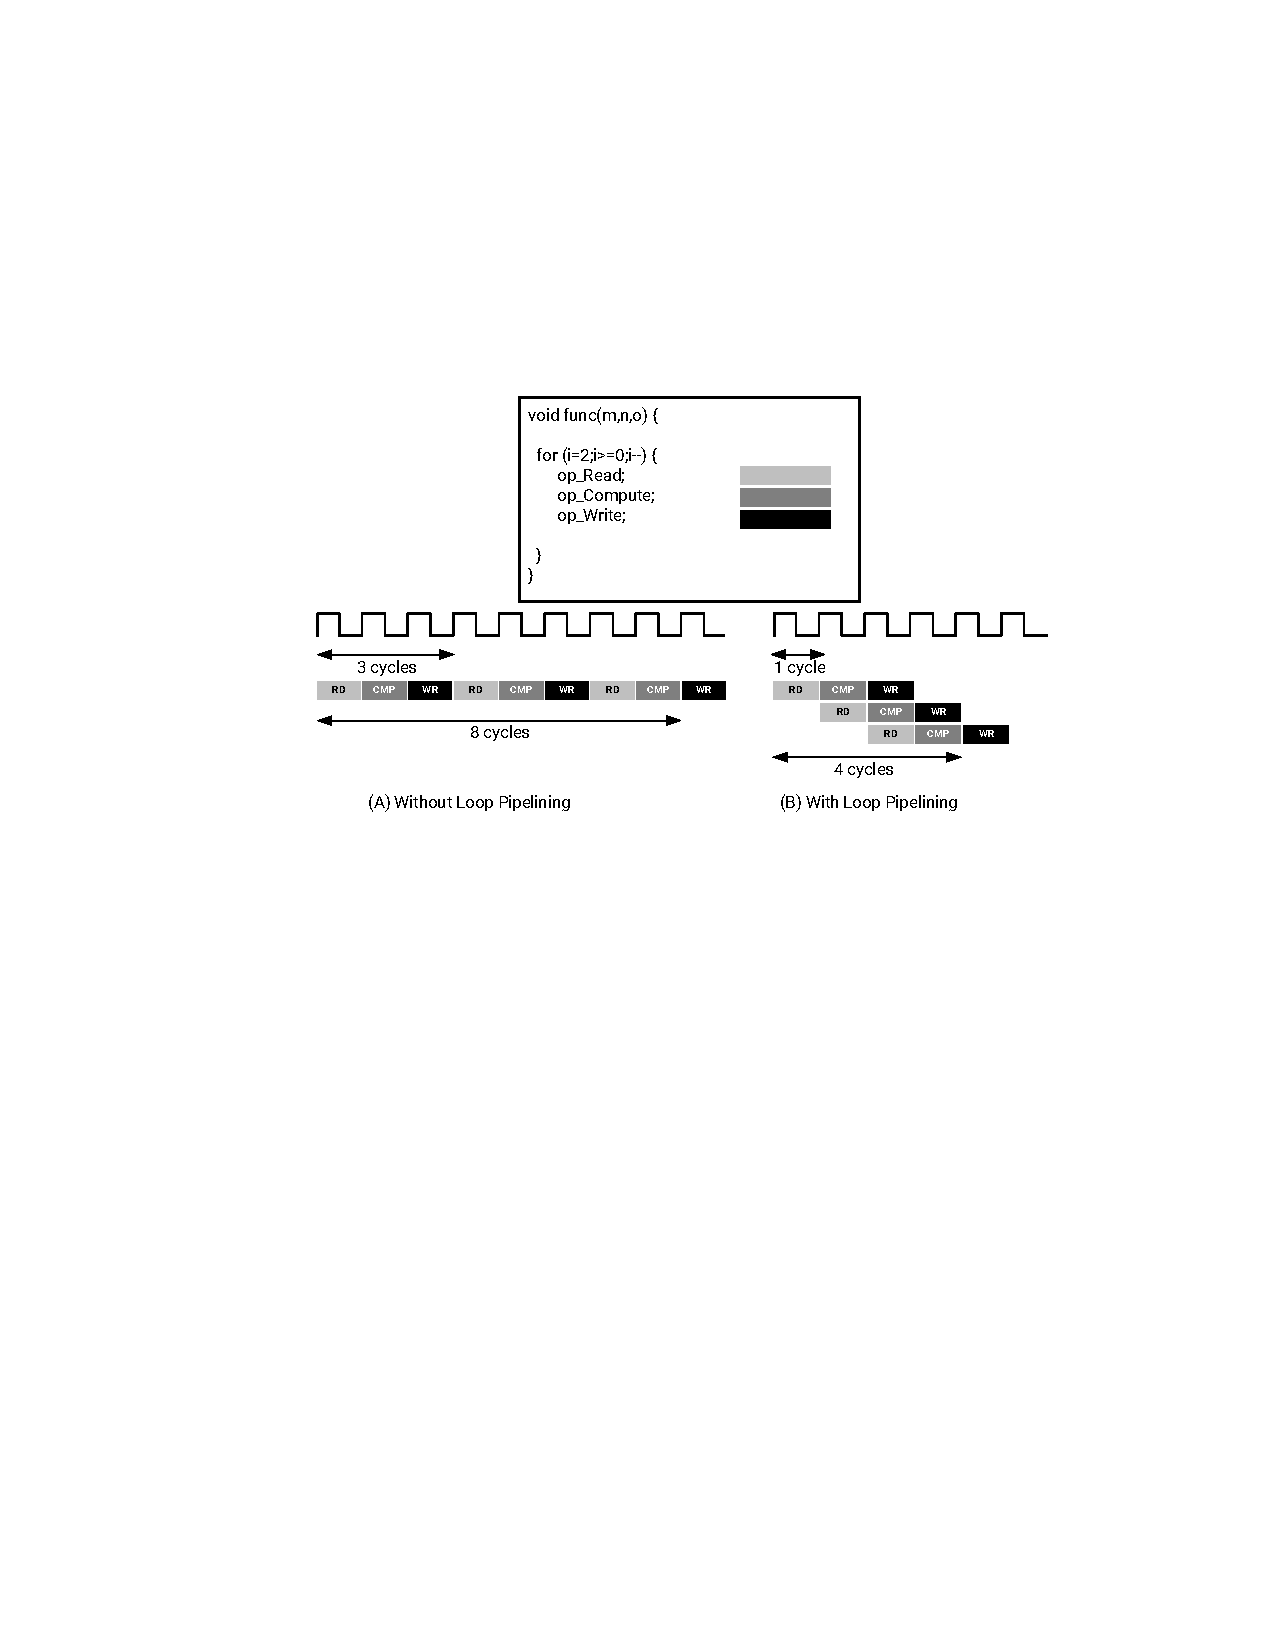
\includegraphics[width=\linewidth]{figures/pragma_pipeline.pdf}
    \caption{指令级别流水线示意图}
    \label{fig:pragma_pipeline}
\end{figure}
\begin{figure}[htbp]
    \centering
    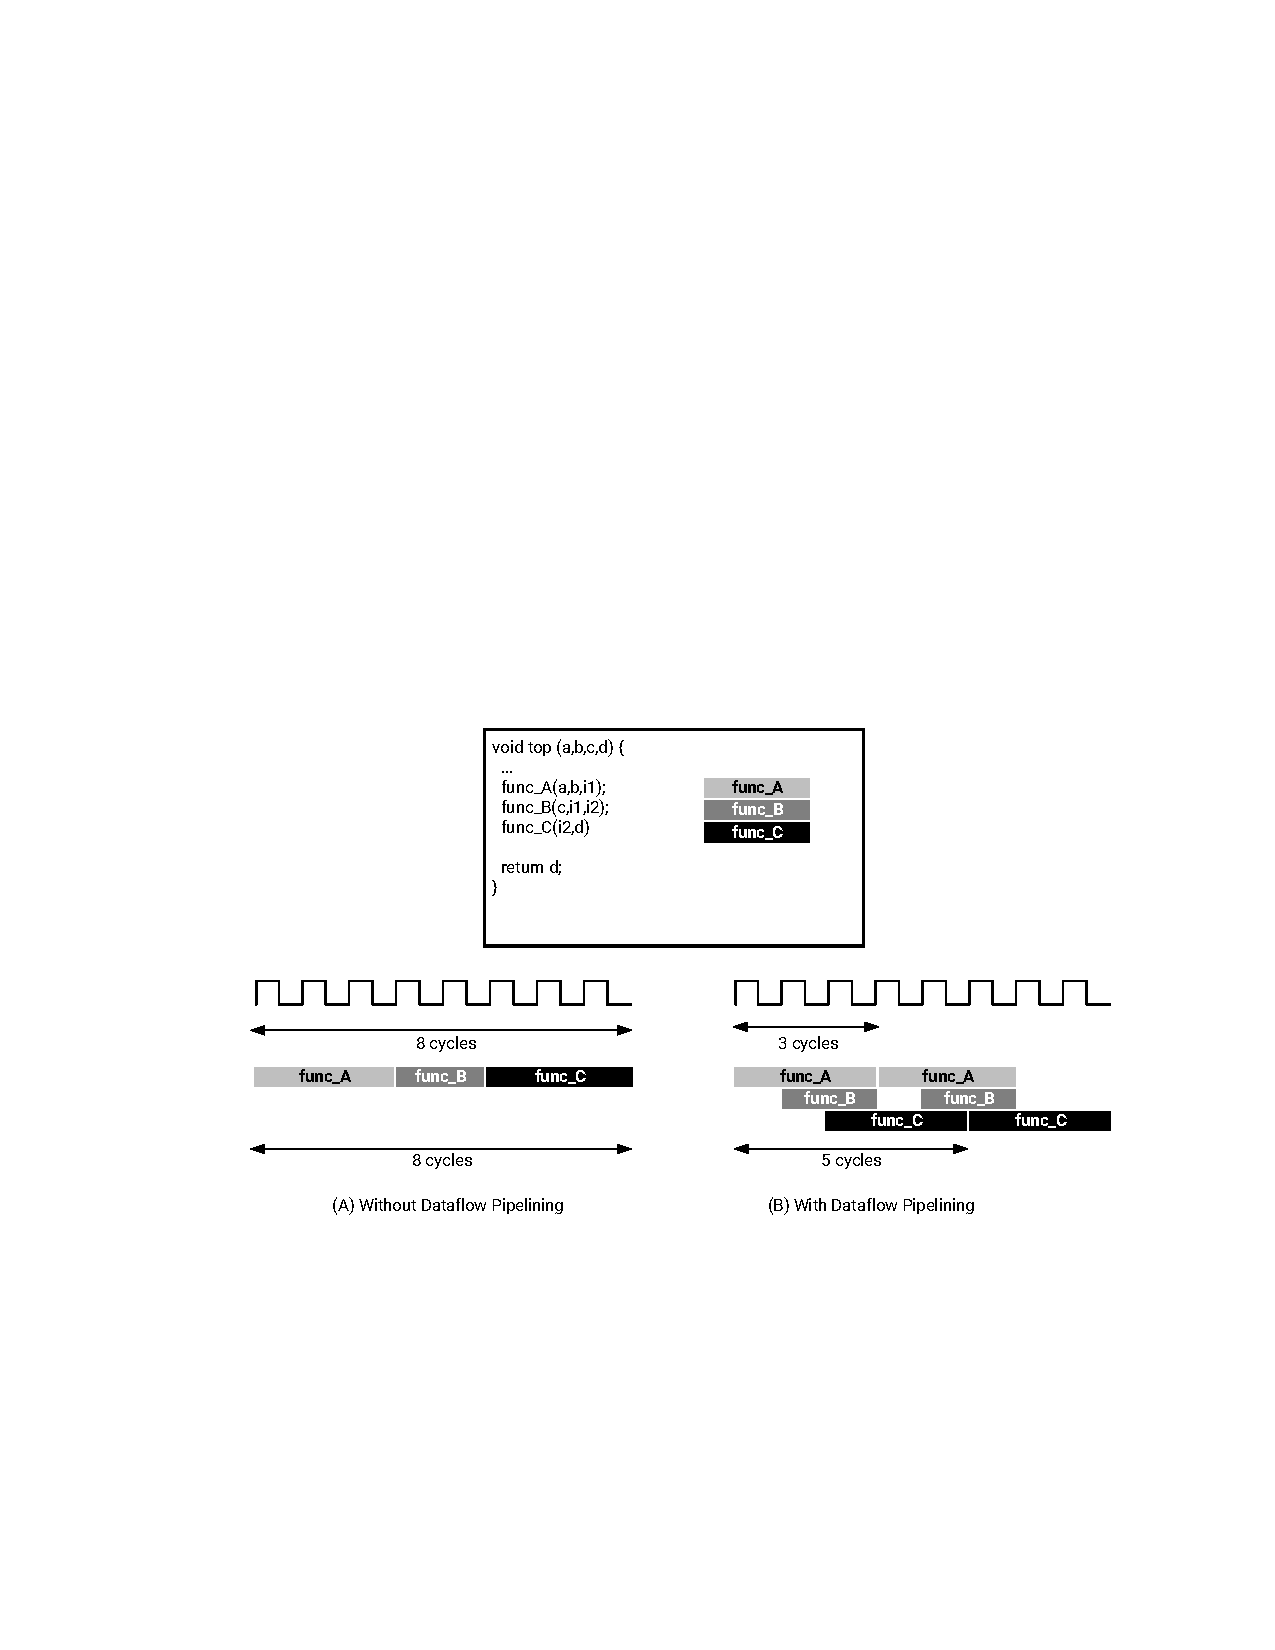
\includegraphics[width=\linewidth]{figures/pragma dataflow.pdf}
    \caption{任务级别流水线示意图}
    \label{fig:pragma_dataflow}
\end{figure}
\subsubsection{指令级别流水线}
在HLS当中,我们可以使用\verb|#pragma HLS pipeline|来实现指令级别的流水化,如图\ref{fig:pragma_pipeline}\footnote{Xilinx Inc. Vitis High-Level Synthesis User Guide (UG1399), 2022.2\label{ug1399}}所示。在该图所示的例子当中,我们将每个指令的执行过程都分为了RD, CMP, WR三个阶段,加入\verb|#pragma HLS pipeline|以后,我们可以将这三个指令的执行阶段流水化,从而将原本需要9个时钟周期完成的任务减少到5个时钟周期。


\subsubsection{任务级别流水线}

任务级别的流水线指的架构允许不同的任务同时进行,是一种细粒度更大的流水线,在HLS当中,我们使用\verb|#pragma HLS dataflow|来实现该级别的流水线,如图\ref{fig:pragma_dataflow}\textsuperscript{\ref {ug1399}}所示。在图中所示的例子当中,我们并没有考虑每个函数内部需要执行多少条指令,但是HLS会自动分析是否有可以复用的模块,从而在最大程度上实现多任务流水化。在本例中,加入\verb|#pragma HLS dataflow|以后,我们可以将原本需要8个时钟周期完成的任务减少到5个时钟周期。

\subsection{数组优化}
\subsubsection{数组分区(Array Partitioning)}
\begin{figure}[htbp]
    \centering
    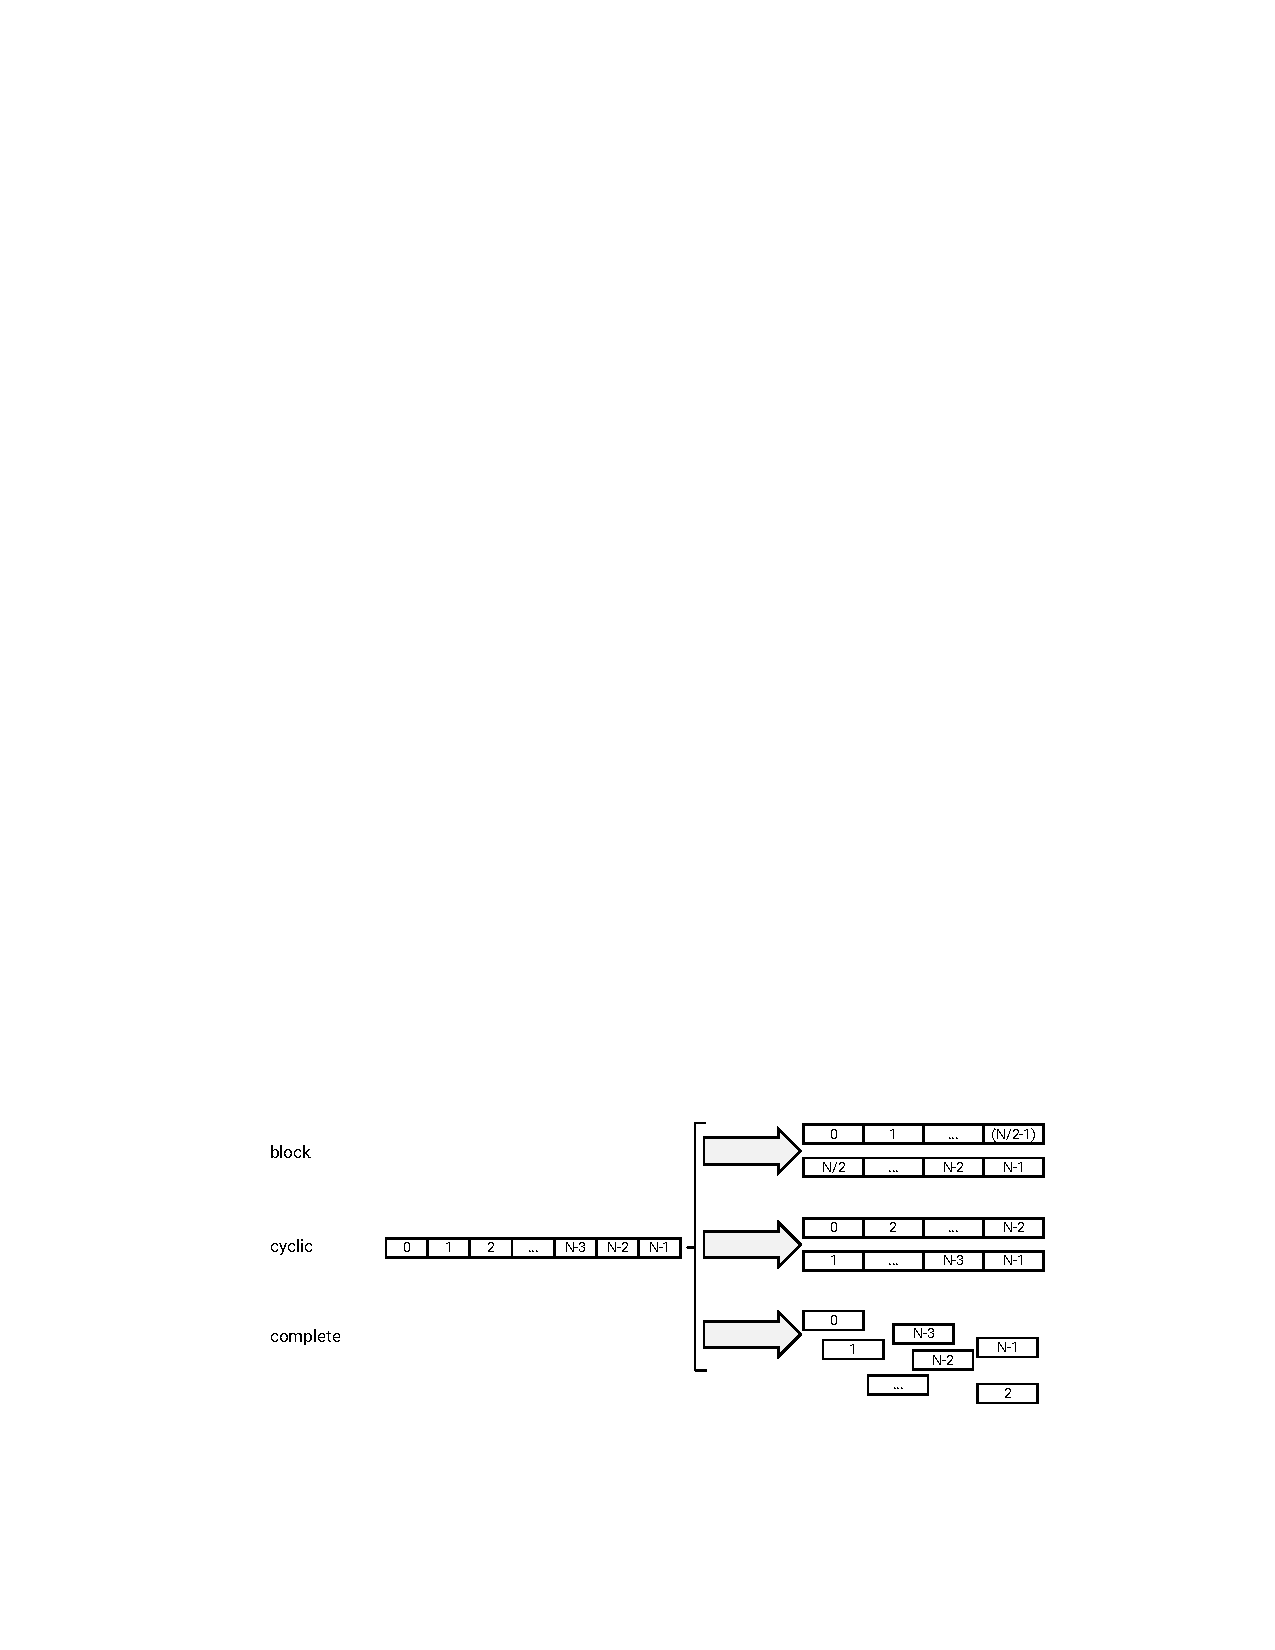
\includegraphics[width=\linewidth]{figures/array_partitioning.pdf}
    \caption{三种数组分区方式示意}
    \label{fig:array_partitioning}
\end{figure}
在Vitis HLS当中,如果定义一个数组,HLS会默认将其编译成一个双口RAM,允许一个线程写一个线程读。但如果想对该数组进行同时写或者同时读等并行的操作,就会受到极大的限制。数组分区的功能就是将一个数组分割成多个小块数组,在编译时体现为将一个RAM块分割成多个小的RAM块或者寄存器,从而实现对数组的并行操作。

Vitis HLS提供了三种数组分区的方式:block, cyclic, complete。block将原数组分割成多个相同大小的块,在原数组中的相邻元素在块内也是相邻的;cyclic也将原数组分割成相同大小的块,但是元素为交错排列;complete将原数组完全打散,变成独立的元素,相当于将RAM形式转换成了寄存器形式。三种分区方式如图\ref{fig:array_partitioning}所示。

\subsubsection{数组重组(Array Reshaping)}
\begin{figure}[htbp]
    \centering
    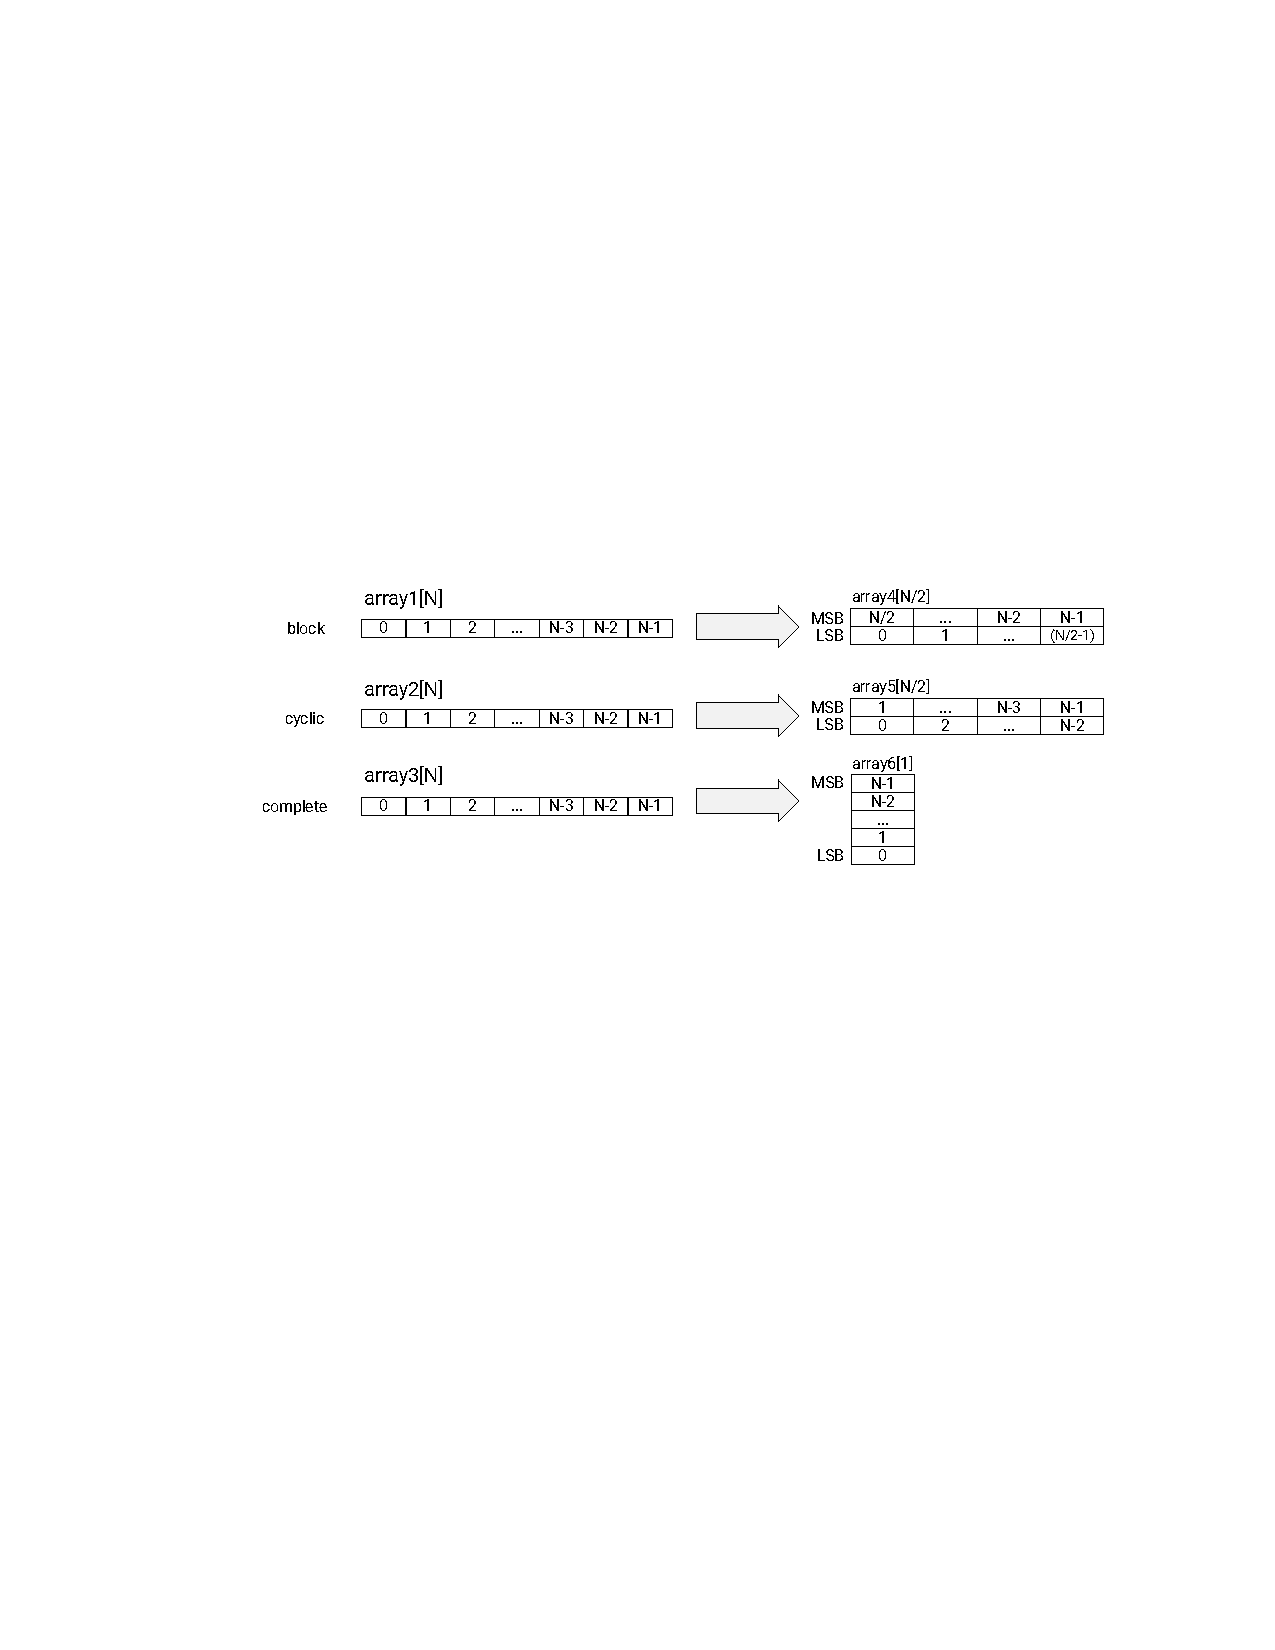
\includegraphics[width=\linewidth]{figures/array_reshaping.pdf}
    \caption{三种数组重组方式示意}
    \label{fig:array_reshaping}
\end{figure}

数组重组旨在能够在单个时钟周期内能够读取更多的数据。同时减少BRAM的使用数量以及并行读取数据\cite{noauthor_vitis_2022}。和数组分区类似,数组重组也有block, cyclic和complete三种方式,如图\ref{fig:array_reshaping}所示。




